En este capítulo procederemos a detallar la planificación que ha seguido el pro-
yecto. En particular, se describe las etapas por las que
ha pasado el proyecto, la planificación temporal y la organización del personal
involucrado.

En general, el desarrollo del proyecto se ha ajustado razonablemente bien al calendario
inicialmente dispuesto en la planificación, con algunas etapas durando
más de lo previsto pero otras terminando antes de lo planificado.

\section{Fase inicial}

La primera fase consistió en plantear la idea del proyecto, con la ayuda del tutor. Tras plantear
varios enfoques, se decidió realizar este proyecto debido a las motivaciones escritas anteriormente.

También se pensó en que lenguaje se desarrollaría el proyecto, así como las principales bibliotecas que
se usarían durante la realización del mismo, priorizando siempre opciones libres. Finalmente se optó por
utilizar el lenguaje Python por su documentación, comunidad y amplia biblioteca estándar.

\section{Fase de análisis}

Esta etapa está dividida principalmente en las dos partes siguiente:

\begin{itemize}
\item Especificación de los requisitos: estudio de los requisitos que deberá cumplir el proyecto.
\item Recursos necesarios: recursos necesarios que deberemos usar durante el desarrollo del proyecto.
\end{itemize}

\section{Fase de aprendizaje}

Aunque ya había realizado otros proyectos en Python, decidí dedicarle tiempo a perfeccionar mis conocimientos
sobre el lenguaje, así como de la librería estándar y las posibles bibliotecas que me serían útiles en el desarrollo.

Esta fase se caracterizó por intentar entender código ya escrito así como leer tutoriales y documentación
oficial. Se podría dividir en estas etapas:

\begin{itemize}
\item \textbf{Perfeccionamiento del lenguaje Python}: investigar sobre el propio lenguaje, biblioteca estándar
así como metodologías a utilizar.
\item \textbf{Aprendizaje de otras bibliotecas}: investigar bibliotecas externas desarrolladas por la comunidad y
que podrían ser útiles en el desarrollo.
\item \textbf{Investigar sobre lenguajes de marcado}: dado que el usuario escribirá el contenido de la web en ficheros
de texto plano y haciendo uso de lenguaje de marcado. Invertí tiempo en ver cuales eran los más usados, para así poder
darles soporte en la herramienta.
\end{itemize}

\section{Fase de desarrollo}

Tras la consecución de las etapas anteriores, se comenzó el desarrollo del proyecto. Esta etapa del desarrollo 
es la más extensa de todas, como es comprensible. Y me fue posible llevarla a cabo gracias a los
prototipos que iba implementando conforme aprendía.

\begin{itemize}
\item \textbf{Generador básico}: Como primer paso se realizó un generador básico de ficheros a partir 
de ficheros de texto plano. Esto incluía la generación estructural de toda la web resultante.
\item \textbf{Adaptar sistema de plantillas}: Otro de los aspectos más importantes fue adaptar el sistema 
de plantillas usado (Jinja) con el motor de generación de forma que los html generados fueran totalmente
personalizables por los usuarios.
\item \textbf{Mejor de output}: Al ser una herramienta que se ejecuta por la linea de comandos, se invirtió
bastante tiempo en que el output ofrecido al usuario fuera realmente verbose y útil, dando información relevante.
\item \textbf{Internacionalización}: Sistema de internacionalización fácil e intuitivo de usar, que permitirá al usuario
escribir plantillas HTMLs una única vez para todos los idiomas configurados.
\item \textbf{Ampliación de funcionalidades}: una vez que ya se había desarrollado toda las funcionalidades básicas,
se dedico tiempo a mejorar las ya existentes, así como a implementar nuevas.
\end{itemize}


\section{Pruebas y correcciones}

Una de las etapas más importantes del desarrollo de cualquier proyecto. Esta etapa se realizó en paralelo
a la de desarrollo, ya que conforme se implementaron nuevas funcionalidades, se iban probando exhaustivamente 
bajo el contexto de las distintas situaciones que pudiera darse, hasta obtener el comportamiento
esperado.

\section{Redacción de la memoria}

La redacción de la memoria se ha redactado conforme se iba avanzando en el desarrollo del proyecto.
Pero tras la finalización de éste, se le ha dedicado más tiempo a su finalización, corrigiendo puntos que
finalmente no se han adecuado al producto final.

\section{Diagrama de Gantt}

A continuación se muestra la planificación anteriormente comentada, en su correspondiente diagrama de
Gantt:


\begin{figure}[htbp]
    \centering
    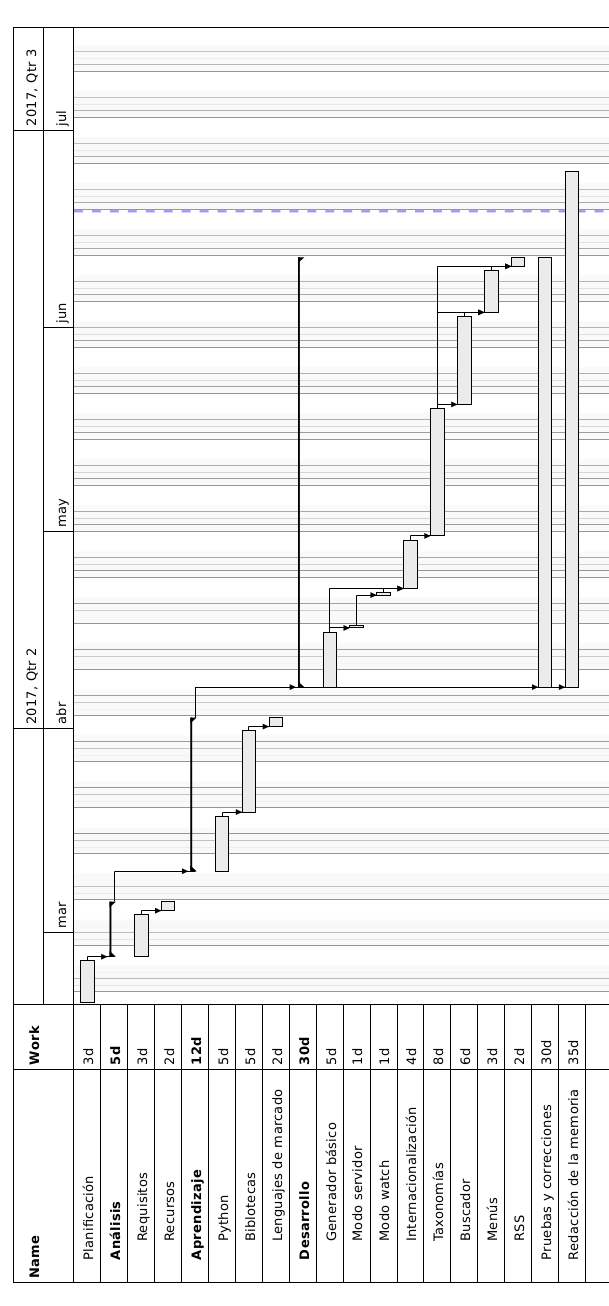
\includegraphics[width=0.7\textwidth]{2_calendario/diagrama_gantt}
    \caption{Diagrama de Gantt}
    \label{fig:gantt}
\end{figure}
